\chapter{Dinámica de Friedmann: materia, radiación y energía del vacío}

\lectureoverview{La cinemática de un universo en expansión puede expresarse en una sola línea: las distancias físicas crecen con un factor de escala \(a(t)\). El problema ahora es determinar esa función. Recuperaremos la ecuación de Friedmann para el espacio plano a partir de la conservación newtoniana de la energía, la resolveremos primero para la materia ordinaria y luego veremos por qué la radiación y la energía del vacío conducen a historias cósmicas completamente distintas.}

\section{La geometría que hay que explicar}

En un instante cósmico dado, el universo a gran escala parece homogéneo e isótropo. Las galaxias, los cúmulos y los supercúmulos son estructuras reales, desde luego, pero a escalas de cientos de millones o miles de millones de años luz, su distribución se vuelve notablemente uniforme. Esta regularidad empírica se denomina principio cosmológico. El nombre no lo convierte en un teorema; la fuerza del principio proviene de la observación.

Hay un segundo hecho empírico. Dentro de la precisión actual, los grandes triángulos espaciales se comportan como triángulos euclidianos. Es útil compararlo con hacer mediciones en un campo de fútbol. Si unas líneas bien tensadas forman triángulos cuyos ángulos suman \(180^\circ\), no se ha demostrado que la Tierra sea plana en su conjunto. Se ha mostrado que el radio de curvatura terrestre es grande en comparación con el campo. La medición cósmica tiene la misma estructura lógica: el espacio puede tener un radio de curvatura muy grande, pero en la región observable se aproxima bien por un espacio plano.

La geometría de referencia es el espacio-tiempo de Minkowski,
\begin{equation}
  d\tau^2=dt^2-\left(dx^2+dy^2+dz^2\right).
  \label{eq:l09-minkowski}
\end{equation}
El corchete es simplemente el elemento de distancia euclidiana en tres dimensiones. En cambio, en la relatividad general, los coeficientes de los diferenciales de coordenadas son campos. Pueden variar con la posición y el tiempo, y también puede haber términos cruzados. Estos coeficientes métricos son los sucesores relativistas del campo gravitatorio newtoniano.

\begin{figure}[H]
  \centering
  \includegraphics[width=0.72\textwidth]{lecture_09_figure_01.png}
  \caption{El elemento de tiempo propio de Minkowski presentado al comienzo de la clase. Fotograma de la fuente en 00:01:50.}
  \label{fig:l09-minkowski-board}
\end{figure}

En un universo en expansión espacialmente plano, la homogeneidad y la isotropía dejan un único factor de escala dependiente del tiempo:
\begin{equation}
  d\tau^2=dt^2-a^2(t)\left(dx^2+dy^2+dz^2\right).
  \label{eq:l09-flat-frw}
\end{equation}
Usamos unidades en las que \(c=1\), de modo que el tiempo y la longitud tienen las mismas dimensiones. Hay dos convenciones coherentes. Se puede asignar a \(x,y,z\) dimensiones de longitud y considerar \(a\) adimensional, o bien tratar \(x,y,z\) como etiquetas adimensionales y dejar que \(a\) tenga dimensiones de longitud. La clase emplea la segunda convención porque hace visible el significado físico de \(a(t)\).

\begin{figure}[H]
  \centering
  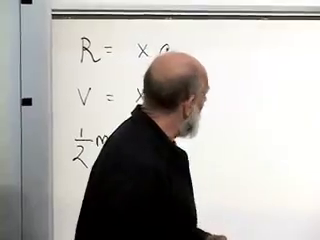
\includegraphics[width=0.72\textwidth]{lecture_09_figure_02.png}
  \caption{La métrica plana en expansión, con el factor de escala multiplicando el elemento de línea espacial euclidiano. Fotograma de la fuente en 00:09:12.}
  \label{fig:l09-expanding-metric-board}
\end{figure}

Imaginemos coordenadas dibujadas sobre una lámina de goma. Las marcas de coordenadas permanecen unidas a la lámina mientras aumenta la distancia física entre ellas. Por tanto, una diferencia de coordenadas como «de \(x=0\) a \(x=1\)» no es más que un par de etiquetas. La distancia que representa ese intervalo es \(a(t)\). Encontrar la ecuación que rige este factor de escala es el problema dinámico de la clase.

\section{Geometrías espaciales cerradas, planas y abiertas}

La planitud es una simplificación observacional, no una consecuencia de la homogeneidad. Hay tres geometrías espaciales homogéneas e isótropas: de curvatura positiva, nula y negativa. Para entender el caso positivo, conviene precisar la dimensión.

El lugar geométrico
\begin{equation}
  X_1^2+X_2^2=R^2
\end{equation}
es un círculo, o una esfera unidimensional \(S^1\). Su interior relleno es un disco, también llamado bola bidimensional. Al añadir una coordenada de inmersión se obtiene
\begin{equation}
  X_1^2+X_2^2+X_3^2=R^2,
\end{equation}
la esfera ordinaria \(S^2\). Al añadir una cuarta coordenada de inmersión se obtiene
\begin{equation}
  X_1^2+X_2^2+X_3^2+X_4^2=R^2,
  \label{eq:l09-three-sphere}
\end{equation}
una esfera tridimensional \(S^3\), que es en sí misma un espacio tridimensional. No podemos visualizar su inmersión en cuatro dimensiones, pero la geometría intrínseca no necesita esa inmersión para existir.

\begin{figure}[H]
  \centering
  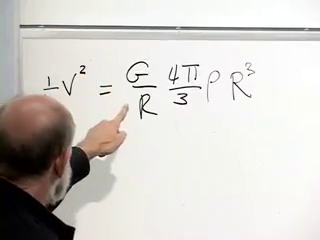
\includegraphics[width=0.72\textwidth]{lecture_09_figure_03.png}
  \caption{La ecuación de inmersión empleada para introducir la esfera tridimensional. Fotograma de la fuente en 00:16:40.}
  \label{fig:l09-three-sphere-board}
\end{figure}

Todos los puntos de una esfera ideal son geométricamente equivalentes, y todas las direcciones en un punto también lo son. Por tanto, una esfera es homogénea e isótropa. Si su radio se multiplica por \(a(t)\), todo el espacio se expande o se contrae sin que se elija un centro en la esfera. Al seguir hacia atrás la evolución de ese universo, no se concentra toda la materia en un lugar especial dentro de un vacío exterior. El espacio entero se hace pequeño, de modo que cada par de puntos se acerca. El Big Bang no es una explosión desde un punto del espacio.

En una esfera de curvatura positiva, la suma de los ángulos de los triángulos geodésicos es mayor que \(180^\circ\). En los triángulos planos, la suma es exactamente \(180^\circ\). En una geometría homogénea de curvatura negativa, representada de manera imperfecta por una silla de montar, la suma es menor que \(180^\circ\). Estas pruebas intrínsecas distinguen los tres casos.

\begin{figure}[H]
  \centering
  \includegraphics[width=0.72\textwidth]{lecture_09_figure_07.png}
  \caption{Curvaturas positiva, nula y negativa ilustradas mediante las formas características de sus triángulos. Fotograma de la fuente en 00:37:30.}
  \label{fig:l09-curvature-board}
\end{figure}

Una métrica local perfectamente plana no demuestra por sí sola que el espacio sea topológicamente infinito. Las topologías planas compactas son matemáticamente posibles, aunque en la clase se adopta el modelo euclidiano infinito más sencillo.
\editorialnote{Esta salvedad sobre la topología global no es necesaria para ninguna de las dinámicas locales que siguen.}

\section{Etiquetas comóviles y ley de Hubble}

Volvamos ahora a la lámina plana en expansión y dibujemos en ella una cuadrícula de coordenadas. En coordenadas comóviles, la cuadrícula se expande junto con el flujo de materia a gran escala. Una galaxia o, más precisamente, un cúmulo de galaxias suficientemente promediado conserva aproximadamente una etiqueta de coordenadas fija, aunque cambie su distancia física respecto de otro objeto comóvil.

\begin{figure}[H]
  \centering
  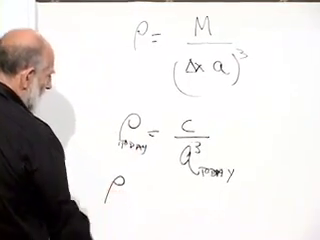
\includegraphics[width=0.72\textwidth]{lecture_09_figure_04.png}
  \caption{Una cuadrícula de coordenadas que acompaña a una lámina espacial en expansión. Fotograma de la fuente en 00:22:20.}
  \label{fig:l09-comoving-grid-board}
\end{figure}

Para dos objetos separados a lo largo del eje \(x\) por un intervalo comóvil fijo \(\Delta x\), su distancia física es
\begin{equation}
  D(t)=a(t)\,\Delta x.
  \label{eq:l09-physical-distance}
\end{equation}
Al derivar manteniendo fijo \(\Delta x\), se obtiene
\begin{equation}
  v(t)=\dot a(t)\,\Delta x
      =\frac{\dot a(t)}{a(t)}D(t).
\end{equation}
Si definimos
\begin{equation}
  H(t)\equiv\frac{\dot a(t)}{a(t)},
  \label{eq:l09-hubble-parameter}
\end{equation}
obtenemos la ley de Hubble,
\begin{equation}
  v=H(t)D.
  \label{eq:l09-hubble-law}
\end{equation}
La palabra «constante» en «constante de Hubble» significa que es constante en el espacio en un instante cósmico dado. No implica que permanezca constante a lo largo de la historia cósmica.

\begin{figure}[H]
  \centering
  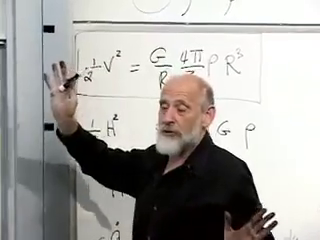
\includegraphics[width=0.72\textwidth]{lecture_09_figure_05.png}
  \caption{La derivación en la pizarra \(D=a\Delta x\),
  \(v=(\dot a/a)D=HD\). Fotograma de la fuente en 00:26:40.}
  \label{fig:l09-hubble-board}
\end{figure}

\begin{classroomqa}\audiencequestion{Si vemos una galaxia distante tal como era en un tiempo anterior, ¿debería su parámetro de Hubble inferido ser realmente igual al valor que medimos hoy en las cercanías?}\lecturerresponse{Solo cuando el tiempo retrospectivo es pequeño en comparación con la edad del universo. A distancias moderadas, \(H(t)\) varía lo bastante poco como para que sea útil un único valor. A distancias verdaderamente cosmológicas observamos épocas anteriores y hay que tener en cuenta la dependencia temporal de \(a\) y \(H\). Esa es una de las razones por las que necesitamos una ecuación dinámica para el factor de escala.}\end{classroomqa}

\section{Rayos nulos en un sistema de coordenadas en expansión}

\begin{classroomqa}\audiencequestion{¿Afecta el factor de escala a la propagación de la luz entre galaxias distantes?}\lecturerresponse{Un rayo de luz sigue una trayectoria nula, así que \(d\tau=0\). Para un rayo que se propaga a lo largo del eje \(x\) positivo, \(dy=dz=0\), y la métrica en expansión da
\begin{align}
  0&=dt^2-a^2(t)dx^2,
  &dt&=a(t)dx,\notag\\
  &&\frac{dx}{dt}&=\frac{1}{a(t)}.
  \label{eq:l09-null-ray}
\end{align}
La velocidad coordenada disminuye a medida que crece \(a(t)\), pero la velocidad física local de la luz sigue siendo \(c=1\). Un intervalo fijo de coordenadas representa una distancia física cada vez mayor.}\end{classroomqa}

\begin{figure}[H]
  \centering
  \includegraphics[width=0.72\textwidth]{lecture_09_figure_06.png}
  \caption{La condición nula y \(dt=a(t)dx\) para la propagación radial de la luz. Fotograma de la fuente en 00:30:54.}
  \label{fig:l09-null-board}
\end{figure}

Se pueden elegir coordenadas en las que este mismo hecho se exprese como «la luz se ralentiza cuanto más lejos está», pero entonces las longitudes y los relojes adquieren descripciones igualmente engorrosas. El lenguaje del espacio en expansión es más claro porque conserva la afirmación local de que todos los observadores en caída libre miden la misma velocidad de la luz.

\begin{classroomqa}\audiencequestion{¿Hay pruebas de que la propagación local de la luz y la física atómica sean iguales en galaxias distantes?}\lecturerresponse{Solo tienen significado operacional las comparaciones adimensionales. Se puede elegir el tamaño de un átomo como unidad de longitud y un período atómico o nuclear como unidad de tiempo, y luego preguntar cuántos de esos períodos necesita la luz para recorrer la longitud elegida. Las observaciones espectrales respaldan la afirmación de que esas razones adimensionales son iguales en regiones distantes. La evidencia es indirecta, pero este es precisamente el tipo de comparación con el que se pone a prueba la uniformidad de las leyes locales.}\end{classroomqa}

Cuando el universo observable era extremadamente pequeño, la luz podía cruzar rápidamente una región física dada, expresada en la unidad correspondiente al tiempo de cruce de la luz. Esto no significa que \(c\) fuera diferente. Significa que la propia región era pequeña.

\section{Una esfera newtoniana dentro del universo}

Pasemos ahora de la cinemática a la dinámica. Situémonos en el origen y tracemos una esfera lo bastante grande para contener muchas galaxias y cúmulos. Elijamos una galaxia en su frontera. En un universo homogéneo, la distribución de masa es esféricamente simétrica a nuestro alrededor, y el teorema de las capas de Newton da dos resultados cruciales:
\begin{enumerate}
  \item toda la materia distribuida esféricamente fuera del radio elegido ejerce una fuerza newtoniana neta nula sobre la galaxia situada en la frontera;
  \item toda la materia dentro de la esfera actúa, para este movimiento radial, como si estuviera concentrada en el centro.
\end{enumerate}
Usamos un sistema de referencia en el que estamos en reposo, de modo que las velocidades y aceleraciones del argumento siguiente se miden respecto de nosotros.

\begin{figure}[H]
  \centering
  \includegraphics[width=0.72\textwidth]{lecture_09_figure_08.png}
  \caption{Construcción basada en el teorema de las capas: nosotros en el centro y una galaxia de prueba en la frontera de una gran esfera homogénea. Fotograma de la fuente en 00:41:10.}
  \label{fig:l09-shell-board}
\end{figure}

\begin{figure}[H]
  \centering
  \begin{tikzpicture}[scale=0.92,>=Latex]
    \draw[thick] (0,0) circle (2.35);
    \fill (0,0) circle (2pt) node[below left] {us};
    \fill (2.35,0) circle (2.2pt) node[right] {test galaxy \(m\)};
    \draw[->,thick,blue!65!black] (0.18,0) -- (2.15,0)
      node[midway,above] {\(R=a(t)x\)};
    \draw[->,thick,red!65!black] (2.35,0.12) -- (3.25,0.12)
      node[midway,above] {\(v=\dot a(t)x\)};
    \node[align=center,text width=7cm] at (0,-2.85)
      {outside shells cancel;\\enclosed mass acts at the center};
  \end{tikzpicture}
  \caption{Reconstrucción limpia de la construcción newtoniana.}
  \label{fig:l09-shell-clean}
\end{figure}

Si la galaxia tiene una coordenada comóvil fija \(x\), su radio físico y su velocidad son
\begin{equation}
  R(t)=x a(t),
  \qquad
  v(t)=x\dot a(t)=H(t)R(t).
  \label{eq:l09-radius-velocity}
\end{equation}
Sea \(M\) la masa encerrada por la esfera y \(m\) la masa de la galaxia de prueba. La energía newtoniana es
\begin{equation}
  E=\frac12 m v^2-\frac{GMm}{R}.
  \label{eq:l09-newtonian-energy}
\end{equation}

\begin{figure}[H]
  \centering
  \includegraphics[width=0.72\textwidth]{lecture_09_figure_09.png}
  \caption{La secuencia completa de la pizarra: \(R=xa\), \(v=x\dot a\) y la ecuación de la energía newtoniana particularizada para \(E=0\). Fotograma de la fuente en 00:48:40.}
  \label{fig:l09-energy-board}
\end{figure}

La energía puede ser positiva, nula o negativa. Empecemos por el límite entre el escape y el colapso, \(E=0\), para el cual
\begin{equation}
  \frac12 v^2=\frac{GM}{R}.
  \label{eq:l09-zero-energy}
\end{equation}

\begin{classroomqa}\audiencequestion{¿Qué significa que la energía total sea nula para la galaxia que se aleja?}\lecturerresponse{Es exactamente el caso de la velocidad de escape. Una energía positiva significa un movimiento por encima de la velocidad de escape; una energía negativa, un movimiento por debajo de ella y, en el modelo newtoniano con solo materia, un retorno eventual. Empezamos en el límite entre esas posibilidades y volveremos a los otros signos después de derivar la ecuación plana.}\end{classroomqa}

\begin{classroomqa}\audiencequestion{¿Varía la masa encerrada \(M\) a medida que se expande la esfera?}\lecturerresponse{No. La esfera es comóvil, así que las mismas partículas permanecen en su interior. Su volumen físico crece y su densidad disminuye, pero la masa total encerrada permanece fija. Esta distinción entre \(M\) y \(\rho(t)\) es esencial.}\end{classroomqa}

Para una densidad homogénea \(\rho(t)\),
\begin{equation}
  M=\frac{4\pi}{3}\rho(t)R^3.
  \label{eq:l09-enclosed-mass}
\end{equation}
Al sustituir en \eqref{eq:l09-zero-energy} se obtiene
\begin{equation}
  \frac12 v^2
  =\frac{G}{R}\left(\frac{4\pi}{3}\rho R^3\right).
  \label{eq:l09-enclosed-energy}
\end{equation}

\begin{figure}[H]
  \centering
  \includegraphics[width=0.72\textwidth]{lecture_09_figure_10.png}
  \caption{Sustitución de la masa encerrada en la ecuación de energía nula. Fotograma de la fuente en 00:54:16.060.}
  \label{fig:l09-enclosed-mass-board}
\end{figure}

Usando \(v=HR\), encontramos
\begin{align}
  \frac12 H^2R^2
    &=\frac{4\pi G}{3}\rho R^2,\\
  H^2
    &=\frac{8\pi G}{3}\rho.
\end{align}
Así, la ley de expansión espacialmente plana con energía nula es
\begin{equation}
  \boxed{\left(\frac{\dot a}{a}\right)^2
  =\frac{8\pi G}{3}\rho(t)}.
  \label{eq:l09-flat-friedmann}
\end{equation}
La cancelación de \(R^2\) no es accidental. En un universo homogéneo, \(H(t)\) debe tener el mismo valor, sea cual sea la galaxia comóvil elegida como objeto de prueba.

\begin{figure}[H]
  \centering
  \includegraphics[width=0.72\textwidth]{lecture_09_figure_11.png}
  \caption{La cancelación del radio y la relación de Friedmann plana resultante en la pizarra. Fotograma de la fuente en 00:57:30.}
  \label{fig:l09-friedmann-board}
\end{figure}

\begin{classroomqa}\audiencequestion{¿Hay pruebas de la relación de energía nula?}\lecturerresponse{Ambos lados pueden inferirse observacionalmente: \(H\) a partir de los datos de recesión y \(\rho\) contabilizando estrellas, gas, materia oscura y energía del vacío. La comparación en la época de la clase encontró que ambos lados concordaban con una precisión aproximada del uno por ciento. La salvedad es importante: hay que incluir todas las formas de energía, y el análisis posterior de la energía del vacío modifica la interpretación ingenua en términos de la velocidad de escape.}\end{classroomqa}

En unidades \(c=1\), la densidad de masa y la densidad de energía tienen las mismas unidades. Por tanto, el símbolo \(\rho\) denotará la densidad de energía total pertinente para el componente considerado.

\section{Materia ordinaria y ley de dos tercios}

La ecuación \eqref{eq:l09-flat-friedmann} no queda cerrada hasta que sepamos cómo cambia \(\rho(t)\). Primero llenemos una caja rectangular comóvil con partículas no relativistas que se mueven lentamente. Sus dimensiones en coordenadas son fijas, mientras que su volumen físico crece como
\begin{equation}
  V(t)=a^3(t)\,\Delta x\,\Delta y\,\Delta z.
\end{equation}
El número de partículas y la masa en reposo dentro de la caja permanecen fijos, así que
\begin{equation}
  \rho_{\mathrm m}(t)=\frac{C_{\mathrm m}}{a^3(t)}.
  \label{eq:l09-matter-dilution}
\end{equation}
Normalizando respecto de la época actual \(t_0\),
\begin{equation}
  \frac{\rho_{\mathrm m}(t)}{\rho_{\mathrm m,0}}
  =\left(\frac{a_0}{a(t)}\right)^3.
  \label{eq:l09-matter-normalized}
\end{equation}

\begin{figure}[H]
  \centering
  \includegraphics[width=0.72\textwidth]{lecture_09_figure_12.png}
  \caption{Densidad de materia, su dilución \(a^{-3}\) y normalización al valor actual. Fotograma de la fuente en 01:04:47.940.}
  \label{fig:l09-density-board}
\end{figure}

\begin{classroomqa}\audiencequestion{¿Cuál es el orden de magnitud aproximado de la densidad de energía actual del universo, y pueden aportarla por sí solos los átomos ordinarios?}\lecturerresponse{Un recuento de la materia bariónica visible solo da parte de la respuesta. La materia oscura y la energía oscura también deben representarse como masa-energía equivalente. La clase cita una escala aproximada que va desde un átomo hasta unas pocas decenas de equivalentes de masa del hidrógeno por metro cúbico, haciendo hincapié en el orden de magnitud y no en un inventario preciso.}\end{classroomqa}

Sustituyamos \eqref{eq:l09-matter-dilution} en
\eqref{eq:l09-flat-friedmann} y absorbamos en una constante positiva \(C\) todos los factores independientes del tiempo:
\begin{equation}
  \left(\frac{\dot a}{a}\right)^2=\frac{C}{a^3},
  \qquad
  \dot a^2=\frac{C}{a}.
  \label{eq:l09-matter-ode}
\end{equation}
Hay dos maneras claras de resolverla. Una solución de prueba en forma de ley de potencias, \(a=K t^p\), exige que
\begin{equation}
  p-1=-\frac{p}{2},
  \qquad p=\frac23.
\end{equation}
De manera equivalente, tomemos la rama positiva de la raíz cuadrada, correspondiente a la expansión, e integremos:
\begin{equation}
  a^{1/2}\frac{da}{dt}=\sqrt C,
  \qquad
  \int a^{1/2}da=\sqrt C\int dt,
\end{equation}
por lo que, al elegir el origen temporal del Big Bang,
\begin{equation}
  a^{3/2}\propto t,
  \qquad
  \boxed{a(t)\propto t^{2/3}}.
  \label{eq:l09-matter-solution}
\end{equation}
En la derivación en directo se pierde brevemente un factor al ajustar los coeficientes; luego se vuelve a la integral y se comprueba el exponente. Los apuntes conservan la comprobación, pero muestran solo el álgebra corregida.

\begin{figure}[H]
  \centering
  \includegraphics[width=0.72\textwidth]{lecture_09_figure_13.png}
  \caption{La solución de prueba en forma de ley de potencias y el exponente enmarcado \(p=2/3\). Fotograma de la fuente en 01:13:05.}
  \label{fig:l09-matter-solution-board}
\end{figure}

Al derivar la solución se obtiene
\begin{equation}
  H(t)=\frac{\dot a}{a}=\frac{2}{3t}.
  \label{eq:l09-matter-hubble}
\end{equation}
El parámetro de Hubble era mayor en el pasado. Por consiguiente, si miramos lo bastante lejos como para observar un tiempo retrospectivo apreciable, no deberíamos prolongar la relación lineal local usando sin cambios el valor actual de \(H_0\).

\begin{figure}[H]
  \centering
  \includegraphics[width=0.72\textwidth]{lecture_09_figure_14.png}
  \caption{Tomar \(\dot a/a\) para \(a\propto t^{2/3}\) da
  \(H=2/(3t)\). Fotograma de la fuente en 01:20:42.}
  \label{fig:l09-hubble-time-board}
\end{figure}

\section{El signo de la energía y la curvatura espacial}

El razonamiento newtoniano nos ha llevado hasta el caso plano de energía nula. La relatividad general añade un hecho que no se puede obtener solo del teorema de las capas: el signo de la energía específica de tipo newtoniano corresponde al signo de la curvatura espacial.
\begin{center}
\begin{tabular}{@{}>{\raggedright\arraybackslash}p{0.20\linewidth}
                    >{\raggedright\arraybackslash}p{0.29\linewidth}
                    >{\raggedright\arraybackslash}p{0.37\linewidth}@{}}
  \toprule
  Energía total & Curvatura espacial & Evolución con solo materia \\
  \midrule
  positiva & negativa (abierta) &se expande para siempre \\
  nula &nula (plana) &se aproxima al límite de escape \\
  negativa &positiva (cerrada) &se expande, alcanza un máximo y vuelve a colapsar \\
  \bottomrule
\end{tabular}
\end{center}
La última columna supone que no hay energía del vacío. En la analogía del proyectil, una energía positiva significa superar la velocidad de escape; una energía nula, alcanzarla exactamente; y una energía negativa, quedar por debajo de ella. Las ecuaciones de Einstein identifican estos tres casos, respectivamente, con geometrías espaciales abiertas, planas y cerradas.

\section{Fotones y ley de un medio}

La ley de la materia \(\rho\propto a^{-3}\) supone que la energía de cada partícula es aproximadamente fija mientras disminuye la densidad numérica. Los fotones no cumplen esa hipótesis. Para un fotón,
\begin{equation}
  E=h\nu=\frac{hc}{\lambda}.
\end{equation}
La expansión estira su longitud de onda en proporción al factor de escala,
\begin{equation}
  \lambda\propto a,
  \qquad E\propto a^{-1}.
\end{equation}
La densidad numérica de fotones sigue disminuyendo como \(a^{-3}\), y la energía de cada fotón aporta un factor adicional de \(a^{-1}\). Por tanto,
\begin{equation}
  \boxed{\rho_{\mathrm r}(t)\propto a^{-4}(t)}.
  \label{eq:l09-radiation-dilution}
\end{equation}

La analogía de la cuerda de guitarra ilustra la situación física. Se pulsa una cuerda y luego se alarga el tramo que vibra: la longitud de onda aumenta y el tono se vuelve más grave. Un modo de fotón en una caja comóvil en expansión se comporta de forma similar. Si se sigue la evolución hacia atrás, la compresión acorta las longitudes de onda y eleva las energías de los fotones.

\begin{figure}[H]
  \centering
  \includegraphics[width=0.72\textwidth]{lecture_09_figure_15.png}
  \caption{La relación de la densidad de materia ampliada en la pizarra hasta la ley de escala de la radiación \(\rho_{\mathrm r}\propto a^{-4}\). Fotograma de la fuente en 01:29:20.}
  \label{fig:l09-radiation-board}
\end{figure}

Al usar \(\rho_{\mathrm r}\propto a^{-4}\) en la ecuación de Friedmann plana, se obtiene
\begin{equation}
  \left(\frac{\dot a}{a}\right)^2=\frac{C_{\mathrm r}}{a^4},
  \qquad
  \dot a\propto a^{-1},
\end{equation}
y, por tanto,
\begin{equation}
  \boxed{a(t)\propto t^{1/2}}.
  \label{eq:l09-radiation-solution}
\end{equation}
Esto crece más lentamente que \(t^{2/3}\). Si retrocedemos lo suficiente en el tiempo, la radiación necesariamente domina sobre la materia ordinaria, porque \(a^{-4}\) aumenta más rápidamente que \(a^{-3}\) cuando \(a\) disminuye. La clase sitúa la transición entre el dominio de la radiación y el de la materia aproximadamente en la época en que el factor de escala era unas mil veces menor que hoy. Antes de esa transición dominaba la radiación; después, durante un largo intervalo, dominó la materia.

\section{Energía del vacío y expansión exponencial}

La energía del vacío tiene un comportamiento de escala opuesto. Su densidad es una propiedad del espacio vacío y no se diluye al expandirse el universo:
\begin{equation}
  \rho_\Lambda=\text{constant}.
  \label{eq:l09-vacuum-density}
\end{equation}
La materia ordinaria y la radiación se vuelven más densas hacia el pasado, mientras que este término no lo hace. Por eso tenía menos importancia en el universo temprano y cobra más importancia a medida que se diluyen los demás componentes. La clase utiliza la estimación entonces vigente según la cual la energía del vacío aporta aproximadamente \(70\%\) de la densidad de energía cósmica actual.

Con \(\rho_\Lambda\) constante, la ecuación \eqref{eq:l09-flat-friedmann} da una tasa de expansión constante
\begin{equation}
  H_\Lambda=\sqrt{\frac{8\pi G}{3}\rho_\Lambda},
  \qquad
  \frac{\dot a}{a}=H_\Lambda.
\end{equation}
Por tanto,
\begin{equation}
  \boxed{a(t)=a(t_i)e^{H_\Lambda(t-t_i)}}.
  \label{eq:l09-vacuum-solution}
\end{equation}

\begin{figure}[H]
  \centering
  \includegraphics[width=0.72\textwidth]{lecture_09_figure_16.png}
  \caption{La ecuación de densidad constante que conduce a la expansión exponencial. Fotograma de la fuente en 01:35:48.}
  \label{fig:l09-vacuum-board}
\end{figure}

A la escala observada citada en la clase, el universo duplica su tamaño lineal en unos diez a doce mil millones de años. El origen de esta pequeña pero no nula densidad del vacío sigue sin explicación; su existencia y su efecto sobre la expansión son hechos empíricos.

\begin{classroomqa}\audiencequestion{¿En este análisis, la energía del vacío es lo mismo que la energía oscura?}\lecturerresponse{Sí. Aquí, «energía oscura» designa una densidad de energía del vacío constante, equivalente a una constante cosmológica. Se pueden imaginar modelos más generales de energía oscura que varíe con el tiempo, pero no forman parte de los cálculos de esta clase.}\end{classroomqa}

\section{Cómo el universo en expansión desplaza al rojo la luz}

\begin{classroomqa}\audiencequestion{¿Cómo pueden saber los fotones que hemos elegido coordenadas comóviles en expansión y, por eso, reducir su energía?}\lecturerresponse{No responden a nuestras etiquetas. Se propagan por una geometría en la que cambian las distancias físicas. Un tren de ondas que ocupa una región cuyo tamaño físico se duplica adquiere el doble de longitud de onda. Las coordenadas comóviles simplemente describen ese estiramiento de manera económica; no lo causan.}\end{classroomqa}

\begin{classroomqa}\audiencequestion{¿De dónde provienen los fotones de fondo que nos llegan hoy?}\lecturerresponse{Mirar más lejos es mirar hacia épocas anteriores. Al final llegamos a la época en que el material cósmico era un plasma ionizado, opaco porque los fotones se dispersaban repetidamente en partículas cargadas libres. La frontera desde la que los fotones pudieron viajar libremente hasta nosotros por última vez aparece como una esfera que rodea al observador: la superficie de última dispersión.}\end{classroomqa}

\begin{figure}[H]
  \centering
  \includegraphics[width=0.72\textwidth]{lecture_09_figure_17.png}
  \caption{Esquema centrado en el observador de la superficie de última dispersión y de capas cada vez más distantes. Fotograma de la fuente en 01:42:05.}
  \label{fig:l09-last-scattering-board}
\end{figure}

\begin{figure}[H]
  \centering
  \begin{tikzpicture}[scale=0.9,>=Latex]
    \fill (0,0) circle (2pt) node[below] {observer};
    \draw[thick,orange!70!black] (0,0) circle (2.55);
    \node[orange!70!black,align=center] at (0,3.05)
      {surface of last scattering};
    \foreach \a in {25,75,145,210,285,335}{
      \draw[->,blue!60!black] ({2.55*cos(\a)},{2.55*sin(\a)}) --
        ({1.7*cos(\a)},{1.7*sin(\a)});
    }
    \draw[decorate,decoration={snake,amplitude=1.5pt,segment length=7pt},
      red!65!black,thick,->] (-2.5,0) -- (-0.15,0);
    \node[red!65!black,below] at (-1.35,-0.15)
      {redshifted photon};
  \end{tikzpicture}
  \caption{Reconstrucción limpia de la imagen de la última dispersión.}
  \label{fig:l09-last-scattering-clean}
\end{figure}

La radiación se emitió con un espectro característico de un plasma caliente y nos llega con longitudes de onda aproximadamente mil veces mayores. En el lenguaje Doppler de la clase, la superficie emisora distante se aleja rápidamente y su radiación experimenta un intenso desplazamiento al rojo. En términos geométricos, la onda se estira durante su propagación. Ambas descripciones codifican la misma relación,
\begin{equation}
  1+z=\frac{\lambda_0}{\lambda_{\mathrm{em}}}
      =\frac{a_0}{a_{\mathrm{em}}}.
  \label{eq:l09-cosmological-redshift}
\end{equation}
\editorialnote{La ecuación \eqref{eq:l09-cosmological-redshift} es la forma cuantitativa estándar de las descripciones de estiramiento y efecto Doppler empleadas en la clase.}

En una época de observación anterior, la esfera de última dispersión habría estado más cerca en la imagen correspondiente, y los fotones de fondo observados habrían sufrido un menor desplazamiento al rojo y, por tanto, habrían tenido más energía. A medida que avanza el tiempo cósmico, los fotones que llegan a un observador comóvil desde aquel plasma temprano tienen longitudes de onda cada vez mayores.

\section{¿Adónde va la energía de un fotón desplazado al rojo?}

\begin{classroomqa}\audiencequestion{Un fotón se emite con una energía \(h\nu_{\mathrm{em}}\) y llega con desplazamiento al rojo y menos energía. ¿Qué ocurrió con la diferencia?}\lecturerresponse{La derivación newtoniana comenzó como una ecuación de energía. Su forma cosmológica relaciona la tasa de expansión con la densidad de energía de la materia, así que no se pueden tratar la energía de la materia y la expansión como magnitudes conservadas por separado. La clase describe la energía perdida por el fotón como incorporada al balance cinético de la expansión. Un pistón lleno de radiación concreta la analogía: la presión de radiación empuja el pistón hacia fuera, las longitudes de onda de los fotones aumentan y la energía que pierden se convierte en trabajo mecánico y energía cinética del pistón.}\end{classroomqa}

\begin{figure}[H]
  \centering
  \includegraphics[width=0.72\textwidth]{lecture_09_figure_18.png}
  \caption{La pizarra sitúa la ecuación newtoniana de la energía, enmarcada, encima de la ecuación de Friedmann correspondiente. Fotograma de la fuente en 01:44:42.}
  \label{fig:l09-energy-bookkeeping-board}
\end{figure}

\begin{classroomqa}\audiencequestion{¿Qué acopla la energía de la radiación a la expansión?}\lecturerresponse{La presión. En un cilindro con un pistón móvil, los fotones transfieren momento a la pared. Cuando el pistón se mueve, la radiación realiza trabajo; su longitud de onda aumenta y su energía disminuye. El universo homogéneo en expansión no tiene un pistón exterior literal, pero la analogía de \(p\,dV\) explica por qué la densidad de energía de la radiación disminuye más rápidamente de lo que bastaría la mera dilución numérica.}\end{classroomqa}

\begin{figure}[H]
  \centering
  \includegraphics[width=0.72\textwidth]{lecture_09_figure_19.png}
  \caption{El pistón móvil lleno de fotones que se usa para visualizar el trabajo de la presión. Fotograma de la fuente en 01:46:40.}
  \label{fig:l09-piston-board}
\end{figure}

\begin{figure}[H]
  \centering
  \begin{tikzpicture}[scale=0.92,>=Latex]
    \draw[thick] (0,0) rectangle (5.3,2.6);
    \draw[very thick] (4.25,0) -- (4.25,2.6);
    \draw[very thick] (4.25,1.3) -- (5.25,1.3);
    \draw[->,thick,red!65!black] (5.25,1.3) -- (6.2,1.3)
      node[right] {moving piston};
    \foreach \y in {0.55,1.3,2.05}{
      \draw[decorate,decoration={snake,amplitude=1.4pt,segment length=6pt},
        blue!65!black,->] (0.35,\y) -- (3.9,\y);
    }
    \node at (2.15,-0.45) {radiation does \(p\,dV\) work};
  \end{tikzpicture}
  \caption{Reconstrucción limpia de la analogía del pistón con radiación.}
  \label{fig:l09-piston-clean}
\end{figure}

La energía en relatividad general exige cautela. En un espacio-tiempo genérico en expansión no tiene por qué existir una energía global conservada única, análoga a la energía de un sistema newtoniano aislado. La conservación local del tensor de energía-momento sigue cumpliéndose y, para un fluido homogéneo, da lugar a la ecuación de continuidad
\begin{equation}
  \dot\rho+3H(\rho+p)=0,
  \label{eq:l09-continuity}
\end{equation}
que contiene el término de trabajo de presión que subyace a las leyes de escalamiento de la materia y la radiación.\editorialnote{La ecuación \eqref{eq:l09-continuity} es la formulación local precisa de la relatividad general que fundamenta la analogía deliberadamente newtoniana de la clase para llevar la contabilidad de la energía.}

La energía del vacío vuelve especialmente agudo el problema. Como su densidad permanece constante mientras el volumen crece, la energía total del vacío en una región comóvil aumenta. Su presión negativa forma parte de la fuente gravitatoria e impulsa la expansión acelerada. Por lo tanto, no se debe exigir la conservación por separado de la ingenua «energía de la materia en una caja comóvil» sin tener en cuenta la geometría y el trabajo de presión.

\section{Por qué se puede eliminar el factor de escala del término temporal}

\begin{classroomqa}
\audiencequestion{¿Por qué el factor de escala multiplica la parte espacial de la métrica, pero no la parte temporal?}
\lecturerresponse{Se trata de una elección de coordenada temporal. Supongamos que se parte de una coordenada de tiempo conforme \(t\), con
\begin{equation}
  d\tau^2=A^2(t)\left(dt^2-dx^2\right).
\end{equation}
Definamos un nuevo tiempo cósmico \(T\) mediante
\begin{equation}
  dT=A(t)\,dt.
\end{equation}
Entonces
\begin{equation}
  d\tau^2=dT^2-A^2\bigl(t(T)\bigr)dx^2.
\end{equation}
El factor común delante del diferencial temporal ha desaparecido, mientras que el factor de escala físico permanece en el término espacial.}
\end{classroomqa}

\begin{figure}[H]
  \centering
  \includegraphics[width=0.72\textwidth]{lecture_09_figure_20.png}
  \caption{La redefinición del tiempo \(dT=A(t)dt\) que convierte el tiempo conforme en tiempo cósmico. Fotograma de la fuente en 01:51:05.}
  \label{fig:l09-time-reparam-board}
\end{figure}

\section{Curvatura, energía del vacío y destino cósmico}

\begin{classroomqa}
\audiencequestion{Si el universo tuviera curvatura positiva, ¿deberíamos ver ya galaxias que se acercan a nosotros?}
\lecturerresponse{No necesariamente. Un proyectil lanzado por debajo de la velocidad de escape primero se aleja, alcanza un punto de retorno y solo después cae de vuelta. Observamos el universo durante una fase de expansión. Sin energía del vacío, un universo de materia con curvatura positiva acabaría colapsando de nuevo. Una energía del vacío positiva suficientemente grande impide ese punto de retorno, y el valor observado parece lo bastante grande como para que la expansión a largo plazo sea exponencial, independientemente de una pequeña curvatura espacial.}
\end{classroomqa}

El futuro exponencial no es un paraíso energético. Las estrellas acabarán apagándose, las densidades de materia y radiación disminuirán exponencialmente y regiones distantes quedarán fuera del contacto causal. La energía del vacío permanece mientras las estructuras ordinarias se vuelven progresivamente más frías y menos densas.

\begin{classroomqa}
\audiencequestion{Al mirar más atrás en el tiempo, ¿había más fotones que partículas ordinarias?}
\lecturerresponse{La razón entre el número de fotones y el de bariones ya es enorme: según la estimación de la clase, aproximadamente \(10^{10}\) fotones por barión. Ambos números permanecen aproximadamente constantes en un volumen comóvil. Lo que cambia al retroceder en el tiempo es, sobre todo, la energía de cada fotón. Las energías de los fotones aumentan como \(a^{-1}\), mientras que las masas en reposo no relativistas no cambian. Por eso la radiación domina la densidad de energía en los primeros tiempos, aunque la propia razón entre los números no tenga por qué cambiar.}
\end{classroomqa}

La lección central es que la geometría por sí sola no determina la historia cósmica. La ecuación de Friedmann para un universo plano establece la relación entre la expansión y la densidad de energía, pero el contenido material determina cómo evolucionan con el tiempo. La materia no relativista da \(a\propto t^{2/3}\), la radiación da \(a\propto t^{1/2}\) y la energía constante del vacío produce una expansión exponencial. Esas tres leyes ordenan las sucesivas eras del universo y explican por qué el mismo factor de escala rige las distancias, los corrimientos al rojo y la evolución del parámetro de Hubble.
